\chapter{Реализация, сравнения и эксперименты}\label{ch:evaluation}

\section{Пилотная программная реализация}
Все предложенные в данной работе подходы реализованы в созданном в рамках данной работы Хорн-решателе \theringen{} (\emph{R}egular \emph{In}variant \emph{Gen}erator)\footnote{\url{https://github.com/Columpio/RInGen}}.
Реализация занимает 5200 строк на языке \fsharp{}.
Было принято решение реализовать Хорн-решатель с нуля, не встраиваясь в кодовые базы существующих решателей, поскольку предложенные алгоритмы требуют нетривиальных манипуляций с формулами и результатами других логических решателей.


Общая архитектура реализованного инструмента представлена на рисунке~\ref{fig:ringen-arch}.
Инструмент \theringen{} принимает на вход систему дизъюнктов Хорна с ограничениями в формате SMTLIB2~\cite{BarFT-RR-17}.
После парсинга дизъюнктов выполняется их  упрощение, в частности, устранение равенств, селекторов и тестеров. Затем, в зависимости от поданных Хорн-решателю опций, запускается один из алгоритмов, предложенных в данной работе. Так, <<Модуль замены АТД неинтерпретированными функциями>> реализует алгоритм из главы~\ref{ch:fmf}, а <<Модуль создания декларативного описания автомата над деревьями>>~--- алгоритм из главы~\ref{ch:SyncReg}. Результатом работы каждого из них является формула над неинтерпретированными функциями, которая передаётся в сторонний логический решатель~--- инструмент автоматического доказательства теорем \vampire{} или SMT-решатель \cvc{}.
В итоге инструмент возвращает безопасный индуктивный инвариант, если система безопасна, в противном случае~--- резолютивное опровержение.
\begin{figure}[h]
% https://online.visual-paradigm.com/share.jsp?id=323637353533352d31
    \centering
    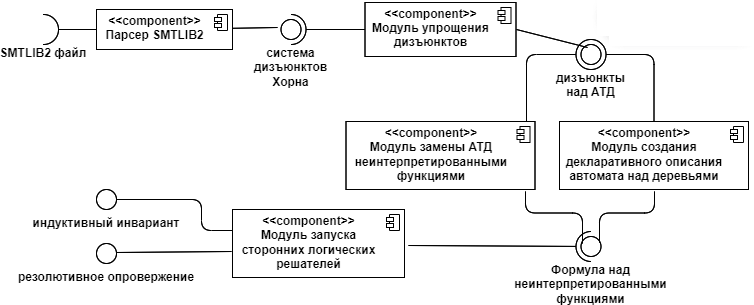
\includegraphics[width=\textwidth]{Dissertation/images/arch.png}
    \caption{Архитектура Хорн-решателя \theringen{}}
    \label{fig:ringen-arch}
\end{figure}


\textbf{\theringen{}.}\label{sec:ringen-pure}
Подход, представленный в главе~\ref{ch:fmf}, реализован автором данного исследования в рамках Хорн-решателя \theringen{}.
Как сам подход, так и его реализация подразумевают использование стороннего SMT-решателя $\verifier$ для теории неинтерпретированных функций с кванторами, поэтому предлагаемая реализация в дальнейшем будет обозначаться $\ringen{\verifier}$.
В частности, в качестве решателя $\verifier$ в экспериментах используются инструмент \vampire{}~\cite{reger2017instantiation} и SMT-решатель \cvc{}.
Инструмент \vampire{} использует портфолио-подход~\cite{reger2014challenges}, то есть перебирает различные техники проверки выполнимости формул, построенные на насыщении системы~\cite{kovacs2013first} или на поиске конечных моделей~\cite{10.1007/978-3-319-40970-2_20}.
Инструмент \cvc{} используется в режиме построения конечных моделей\footnote{с опцией \texttt{-{}-finite-model-find}}~\cite{reynolds2013finite}.
Оба инструмента позволяют как доказывать безопасность системы, так и находить контрпримеры.

\textbf{\ringenSync{}.}
Этот подход, представленный в главе~\ref{ch:SyncReg}, реализован как надстройка над $\ringen{\verifier}$.
В качестве стороннего решателя $\verifier$ в экспериментах использовался \cvc{}, поскольку \ringenSync{} порождает символы с большой арностью, которые не поддерживаются инструментом \vampire{}\footnote{\url{https://github.com/vprover/vampire/issues/348\#issuecomment-1091782513}}.
Эта реализация в дальнейшем будет обозначаться \ringenSync{}\footnote{\url{https://github.com/Columpio/RInGen/releases/tag/ringen-tta}}.

\textbf{\theringenCICI{}.}
Данный подход, представленный в главе~\ref{ch:cici}, реализован в рамках кодовой базы Хорн-решателей \racer{}~\cite{10.1145/3498722} (развитие Хорн-решателя \spacer{}~\cite{komuravelli2016smt}, реализованное в логическом решателе \zprover{}\footnote{\url{https://github.com/Columpio/z3/tree/racer-solver-interaction}}) и Хорн-решателя $\ringen{\verifier{}}$\footnote{\url{https://github.com/Columpio/RInGen/releases/tag/chccomp22}}, описанного выше.
Эта реализация в дальнейшем будет обозначаться $\ringenCICI{\verifier{}}$. Далее описаны обе части этой реализации в Хорн-решателях \racer{} и $\ringen{\verifier{}}$, соответственно, которые далее называются \emph{базовыми} относительно инструмента $\ringenCICI{\verifier{}}$.

Хорн-решатель \racer{} разработан Ари Гурфинкелем (Arie Gurfinkel) и Хари Говинд Ведирамана Кришнаном (Hari Govind Vediramana Krishnan) из университета Ватерлоо.
Инструмент \racer{} основан на подходе, называемом достижимость, направляемая свойством (Property-Directed Reachability, PDR)~\cite{komuravelli2016smt}, который можно рассматривать как сложный экземпляр \cegar{}.
PDR строит абстрактные состояния в виде конъюнкции формул (называемых \emph{леммами}) на различных \emph{уровнях} путём итеративного увеличения уровня в цикле.
При этом поддерживаются следующие возможности: если набор лемм $\{\phi_i\}$ был построен на уровне $n$, то $\bigwedge_i \phi_i$ аппроксимирует сверху все состояния, достижимые менее чем за $n$ шагов перехода, и аппроксимирует снизу свойство безопасности.
Таким образом, леммы в PDR выполняют требование абстракции в процедуре \RunBlackBox{} (листинг~\ref{code:runblackbox}).
Хорн-решатель \racer{} был модифицирован в рамках данного диссертационного исследования таким образом, чтобы в конце каждой итерации набор лемм последнего уровня асинхронно передавался новому процессу инструмента $\ringen{\verifier{}}$.

Процедура \RunBlackBox{} (листинг~\ref{code:runblackbox}) реализована на основе инструмента  $\ringen{\verifier{}}$. Было выполнено  следующее обобщение в процедуре $\substituteLemmas(\prog, a)$ (см.~\autoref{sec:subst_lemmas}).
Конъюнктивная форма лемм инструмента \racer{} используется для вывода инвариантов более общего вида:
$\bigwedge_i(\phi_i(\overline{x})\,\lor\,\overline{x}\!\in\!L_i)$.
Так, имея $a(P) = \bigwedge_i \phi_i$,
мы заменяем все атомы $P(\overline{t})$ на \emph{конъюнкцию дизъюнкций} $\bigwedge_i (\phi_i(\overline{t})\lor L_i(\overline{t}))$ с новыми предикатными символами $L_i$.
Это позволяет выводить более общие инварианты, чем инварианты из объединения классов $\elemclass{}$ и $\abstrDomain$ (см. определение~\ref{def:combined-class}), которое состоит только из формул вида $\phi(\overline{x})\,\lor\,\overline{x}\!\in\!L$.

После преобразований модифицированный $\ringen{\verifier{}}$ вызывает сторонний решатель $\verifier{}$ с ограничением по времени в 30 секунд.
Затем его результаты передаются обратно в Хорн-решатель \racer{}, где они асинхронно обрабатываются.
Кроме того, реализация не выполняет дорогостоящее преобразование в КНФ из листинга~\ref{code:residual-chc}, так как реализация $\ringen{\verifier{}}$ позволяет принимать на вход дизъюнкты Хорна в произвольном виде, поскольку он полагается на сторонний решатель $\verifier{}$ с полной поддержкой логики первого порядка.

\section{Сравнение и соотнесения}\label{ch:relatedWork}

Данный раздел посвящен сравнению предложенных методов решения систем дизъюнктов Хорна с алгебраическими типами данных и существующих методов, реализованных в таких инструментах, как \spacer{}, \racer{}, \eldarica{}, \vericat{}, \hoice{} и \rchc{}. Данные инструменты были отобраны по следующему принципу: инструменты, поддерживающие системы дизъюнктов Хорна над алгебраическими типами данных, которые проверяют как выполнимость, так и невыполнимость этих систем. Так, например, не рассматривались инструменты, решающие родственную проблему автоматизации индукции для теорем с алгебраическими типами данных, такие как, например, \cvc{} в режиме индукции~\cite{reynolds2015induction}, \textsc{AdtInd}~\cite{10.1007/978-3-030-30048-7_35} и пр., поскольку они не принимают на вход системы дизъюнктов Хорна. Также не рассматривались инструменты логического программирование (такие, как \textsc{Prolog}~\cite{ClocksinMellish03}), поскольку они позволяют проверять только невыполнимость систем дизъюнктов Хорна и ничего не говорят об их выполнимости.

\begin{table} [htbp]
    \centering\small
    \begin{threeparttable}% выравнивание подписи по границам таблицы
        \caption{Сравнение Хорн-решателей с поддержкой АТД}\label{tab:hornSolvers}%
        \begin{tabular}{| m{50mm} || x{25mm} | x{25mm} | x{25mm} | x{25mm} |}
            \hline
            \hline
Инструмент & Класс\quad\ \ \  инвариантов & Метод & Возвращает инвариант & Полностью автоматический\\\hline\hline
\spacer{} & \elemclass{} & \pdr{} & Да & Да\\
\racer{} & \catelemclass{} & \pdr{} & Нет & Нет\\
\eldarica{} & \sizeelemclass{} & \cegar{} & Да & Да\\
\vericat{} & -- & Трансф. & Нет & Да\\
\hoice{} & \elemclass{} & \ice{} & Да & Да\\
\rchc{}  & \syncRegFlatClass{} & \ice{} & Да & Да\\\hline
\ringen{\cvc} & \regclass{} & Трансф. + \fmf{} & Да & Да\\
\ringen{\vampire} & -- & Трансф. + \satur{} & Нет & Да\\
\ringenSync{} & \syncRegFullClass{} & Трансф. + \fmf{} & Да & Да\\
\ringenCICI{\cvc} & \regelemclass{} & \ourCEGAR{} & Да & Да\\
\ringenCICI{\vampire} & -- & \ourCEGAR{} & Нет & Да\\
            \hline
            \hline
        \end{tabular}
    \end{threeparttable}
\end{table}

В таблице~\cref{tab:hornSolvers} представлены результаты сравнения работе Хорн-решателей~--- существующих (верхний блок) и предложенных в данной (нижний блок). Предложенные Хорн-решатели описаны в предыдущей главе~\ref{ch:evaluation}, реализуемые ими методы описаны в главах~\ref{ch:fmf},~\ref{ch:SyncReg} и~\ref{ch:cici} данной работы. В таблице, для краткости, название \theringen{} сокращено до \theringen{}, так, например, Хорн-решатель \ringenSync{} в таблице представлен как \ringenSync{}. Под словом <<Трансф.>> имеется в виду, что инструмент построен на применении нетривиальных трансформаций к системе; аббревиатура <<FMF>> обозначает применение автоматического поиска конечных моделей (<<finite-model finding>>, см., например,~\cite{10.1007/978-3-319-40970-2_20,reynolds2013finite}); прочерк в столбце <<Класс инвариантов>> означает следующее: несмотря на то, что при выполнимости системы вывод инструмента неявно кодирует её индуктивный инвариант, не существует всюду останавливающейся процедуры, позволяющей этот вывод проверить. Остальные обозначения поясняются в подразделах, посвящённых соответствующим инструментам.

Большинство рассмотренных инструментов отличаются классами, в которых они ищут индуктивные инварианты. Сравнение самих классов инвариантов было приведено в главе~\cref{ch:comparison}. В контексте сопоставления инструментов сравнение их классов инвариантов важно по следующей причине: если инструмент выводит инварианты в некотором классе, то проблема невыразительности этого класса (невозможность выразить определённые типы отношений) превращается в проблему незавершаемости этого инструмента. Иными словами, поскольку ни один из существующих инструментов не проверяет, существует ли \emph{вообще} инвариант для данной системы дизъюнктов Хорна в его классе\footnote{С одной стороны, эта задача по сложности сравнима с самой задачей верификации, а с другой стороны до сих пор ей были посвящены лишь отдельные работы (см., например,~\cite{10.1145/3022187,10.1145/2837614.2837640})}, то в случае отсутствия такового инструмент не будет завершаться.

Далее приведено краткое сравнительное описание существующих инструментов.

\paragraph{Инструмент \spacer{}~\cite{komuravelli2016smt}} строит элементарные модели (класс \elemclass{}). Этот инструмент создан на основе классической разрешающей процедуры для АТД, а также процедуры интерполяции и устранения кванторов~\cite{bjorner2015playing}. Ядром инструмента является подход \spacer{}, который основан на технике, называемой \emph{достижимость, направляемая свойством} \foreignlanguage{english}{(property-directed reachability, \pdr{})}, которая равномерно распределяет время анализа между поиском контрпримеров и построением безопасного индуктивного инварианта, распространяя информацию о достижимости небезопасных свойств и частичные леммы о безопасности. Инструмент позволяет выводить инварианты в комбинации алгебраических и других типов данных, возвращает проверяемые сертификаты. Подход, используемый в инструменте, корректен и полон. Недостатком инструмента является то, что он выражает инварианты в языке ограничений, а потому часто не завершается на проблемах с АТД.

\paragraph{Инструмент \racer{}~\cite{10.1145/3498722}} является развитием инструмента \spacer{}, позволяя выводить инварианты в языке ограничений, расширенном катаморфизмами. Этот язык ограничений обозначен в таблице~\ref{tab:hornSolvers} как \catelemclass{}. \racer{} также наследует все достоинства подхода \spacer{}. Недостатком подхода является то, что он не полностью автоматический, поскольку требует вручную описывать катаморфизмы, что может быть затруднительно на практике, поскольку по заданной проблеме бывает сложно понять, какие катаморфизмы потребуются для её инварианта. Недостатком самого инструмента является то, что он не возвращает какие-либо проверяемые сертификаты с катаморфизмами.

\paragraph{Инструмент \eldarica{}~\cite{8603013}} строит модели с ограничениями размера термов, которые вычисляют общее количество вхождений конструкторов (класс \sizeelemclass{}). Это расширение весьма ограниченно увеличивает выразительность языка ограничений, поскольку введённая функция считает количество всех конструкторов одновременно, поэтому с её помощью невозможно выразить многие свойства, например, ограничение на высоту дерева. Инструмент \eldarica{} использует подход \cegar{} с абстракцией предикатов и встроенный SMT-решатель \princess{}~\cite{princess}, который предоставляет разрешающую процедуру, а также процедуру интерполяции для АТД с ограничениями на размер термов. Эти процедуры построены на сведении данной теории к комбинации теорий неинтерпретируемых функций и линейной арифметики~\cite{hojjat2017deciding}.

\paragraph{Инструмент \vericat{}~\cite{10.1093/logcom/exab090,pettorossi_proietti_2022,10.1007/978-3-030-51074-9_6,angelis_fioravanti_pettorossi_proietti_2018}} обрабатывает условия проверки над теориями линейной арифметики и АТД и полностью устраняет АТД из исходной системы дизъюнктов путём сворачивания (fold), разворачивания (unfold), введения новых дизъюнктов и других трансформаций. После работы инструмента получается система дизъюнктов Хорна без АТД, на которой может быть запущен любой эффективный Хорн-решатель, например, \spacer{} или \eldarica{}. Основным достоинством подхода является тот факт, что он рассчитан на работу с проблемами, где алгебраические типы данных комбинированы с другими теориями. Основные недостатки подхода заключаются в следующем: сам процесс трансформации может также не завершаться, кроме этого из-за трансформации невозможно восстановить инвариант исходной системы, т.\:е. инструмент не возвращает проверяемого сертификата.

\paragraph{Инструмент \hoice{}~\cite{10.1007/978-3-030-02768-1_8}} строит элементарные инварианты с помощью подхода, основанного на машинном обучении, \ice{}~\cite{10.1007/978-3-319-08867-9_5}. Его достоинством является возможность выводить инварианты в комбинации АТД с другими теориями, а также корректность и полнота, и, наконец, способность возвращать проверяемые сертификаты корректности. Его недостатком является то, что он выводит инварианты в невыразительном языке ограничений, а потому часто не завершается.

\paragraph{Инструмент \rchc{}~\cite{haude2020,losekoot_et_al:LIPIcs.FSCD.2023.7}} также использует подход \ice{}; \rchc{} основан на машинном обучении, однако выражает индуктивные инварианты программ над АТД при помощи \emph{автоматов над деревьями}~\cite{tata}. Но из-за сложностей с выражением кортежей термов автоматами, описанных в разделе~\ref{sec:comparison/undef-in-sync}, подход часто оказывается неприменим для простейших примеров, где существуют классические символьные инварианты. 

\paragraph{Выводы.} Подводя итоги сравнения вышеозначенных инструментов и методов, можно сказать следующее. По сравнении с методом инструмента \rchc{} предложенные в данной диссертационной работе подходы являются альтернативными способами вывода регулярных инвариантов и их надклассов. Поэтому они могут быть совмещены с подходом инструмента \rchc{}, чтобы быстрее сходиться к индуктивному инварианту системы, если он существует. В сравнении с методами остальных существующих инструментов, предложенные подходы позволяют выводить инварианты в независимых классах регулярных инвариантов. Поэтому применение предложенных методов совместно с существующими позволит решать больше различных типов задач.

\section{Дизайн эксперимента}
\subsection{Выбор инструментов для сравнения}
В качестве инструментов для сравнения были выбраны \racer{}~\cite{10.1145/3498722} и \eldarica{}~\cite{8603013}~--- Хорн-решатели с поддержкой алгебраических типов данных, лидирующие на соревнованиях \chccomp{}~\cite{De_Angelis_2022}.
Также были выбраны инструменты \cvcind{} (\cvc{} в режиме индукции)~\cite{reynolds2015induction} и \vericat{}~\cite{10.1093/logcom/exab090}.
Несмотря на то, что эти инструменты не строят индуктивные инварианты \emph{явно}, из-за чего невозможно проверить их корректность, их запуск на эквивалентном бенчмарке добавлен в экспериментальное сравнение, поскольку они решают родственную задачу.


В представленных здесь экспериментах не участвовал Хорн-решатель \hoice{}~\cite{10.1007/978-3-030-02768-1_8}, поскольку он работает не быстрее \racer{}~\cite{10.1145/3498722} и при этом ищет инварианты в том же классе инвариантов \elemclass{}.
Другой известный Хорн-решатель \rchc{}~\cite{haude2020} не участвовал в экспериментах, поскольку он работает нестабильно и часто либо завершается с ошибкой, либо возвращает некорректные результаты.

\subsection{Тестовый набор данных}
Эксперименты проводились на наборе данных \emph{TIP} (Tons of Inductive Problems)~\cite{claessen2015tip}, тестового набора с трека соревнования \chccomp{} 2022\footnote{\url{https://github.com/chc-comp/ringen-adt-benchmarks}}, посвящённого алгебраическим типам данных. Набор \emph{TIP} состоит из 454 систем дизъюнктов Хорна, полученных из \haskell{}-программ с АТД и рекурсией.
В тестовом наборе встречаются следующие алгебраические типы данных: списки, очереди, регулярные выражения и целые числа Пеано.

\subsection{Описание тестового стенда}
Эксперименты проводились на платформе StarExec~\cite{stump2014starexec}, имеющей кластер машин Intel(R) Xeon(R) CPU E5-2609 0 @ 2.40GHz и Red Hat Enterprise Linux~7\footnote{\url{https://www.starexec.org/starexec/public/machine-specs.txt}}, с ограничением на процессорное время работы каждого инструмента на одном тесте в 600~секунд и с ограничением по памяти в 16~ГБ.

\subsection{Исследовательские вопросы}

Для постановки экспериментов были поставлены следующие исследовательские вопросы.

\begin{resquest}[Количество решений]\label{rq:conv}
Поскольку основная цель данной работы~--- предложить подходы, позволяющие проверять выполнимость б\textit{о}льшего числа систем, чем аналоги, путём вывода индуктивных инвариантов, ключевыми являются следующие вопросы.
\begin{itemize}
    \item Позволяют ли предложенные подходы проверять выполнимость б\textit{о}льшего числа систем, чем подходы, строящие классические символьные инварианты?
    \item Позволяют ли предложенные подходы проверять выполнимость систем, у которых существуют классические инварианты?
\end{itemize}
\end{resquest}

\begin{resquest}[Производительность]\label{rq:perf}
$ $

\begin{itemize}
    \item Какова производительность инструментов \theringen{} и \ringenSync{} на проблемах, которые смогли решить они, а также существующие инструменты?
    \item Коллаборативный вывод в \theringenCICI{} может потребовать параллельного запуска нескольких экземпляров оракула. Каково влияние параллельного запуска на производительность?
\end{itemize}
\end{resquest}

\begin{resquest}[Значимость класса индуктивных инвариантов]\label{rq:char}
Коллаборативный вывод, реализованный в \theringenCICI{}, теоретически позволяет не только выводить инварианты в большем классе, но и ускорять сходимость поиска классических символьных инвариантов. Какова при этом доля классических символьных инвариантов на всех уникально решённых инструментом \theringenCICI{} проблемах?
\end{resquest}

\section{Анализ результатов экспериментов}

\subsection{Количество решений}

Количество проблем из тестового набора, решённых существующими и предложенными инструментами, представлено в таблице~\ref{table:eval-all}. Над разделяющей чертой находятся существующие инструменты, а предложенные инструменты расположены под ней.

\begin{table}[t]
    \caption{Результаты экспериментов. <<SAT>> обозначает, что система безопасна (есть индуктивный инвариант), <<UNSAT>> обозначает, что система небезопасна.}
    \label{table:eval-all}
    \small
    \centering
    \begin{tabular}{ |l||c|c| }
    \hline\hline
    Инструмент & SAT & UNSAT\\\hline\hline
    \racer{} & 26 & 22\\
    \eldarica{} & 46 & 12\\
    \vericat{} & 16 & 10\\
    \cvcind{} & 0 & 13\\
    \hline
    \ringen{\cvc{}} & 25 & 21\\
    \ringen{\vampire{}} & 135 & 46\\
    \ringenSync{} & 43 & 21\\
    \ringenCICI{\cvc{}} & 117 & 19\\
    \ringenCICI{\vampire{}} & 189 & 28\\
    \hline\hline
    \end{tabular}
\end{table}

%\subsubsection{\theringen{}.}

\textbf{\theringen{}}. На всех 12 проблемах, на которых инструмент \eldarica{} вернул ответ <<UNSAT>>, инструмент \theringen{} завершился с тем же результатом и он нашёл больше контрпримеров.
Инструменты \ringen{\cvc{}}, \ringen{\vampire{}} и \racer{} нашли контрпримеры для 21, 46 и 22 систем дизъюнктов соответственно, при этом каждый из них нашёл несколько уникальных контрпримеров.
Инструмент \ringen{\vampire{}} построил существенно больше <<UNSAT>> результатов, чем другие инструменты, поскольку в нём реализована эффективная процедура вывода опровержений.
Тем самым, несмотря на то, что предложенные алгоритмы спроектированы для поиска большего числа индуктивных инвариантов, они также позволяют находить уникальные контрпримеры.
Далее, инструмент \eldarica{} нашёл 46 инвариантов в противовес 25 и 135 инвариантам, найденным \ringen{\cvc{}} и \ringen{\vampire{}}.
Из них \eldarica{} решила 25 уникальных (не решённых \ringen{\cvc{}}) задач, каждая из которых является формулировкой некоторого свойства порядковых предикатов ($ <, \le,>, \ge $) на числах Пеано.
Эти проблемы легко решаются инструментом \eldarica{}, поскольку порядковые предикаты сами по себе включены в домен верификации \sizeelemclass{} на уровне примитивов.
Тем не менее инструмент \ringen{\cvc{}} решил 13 уникальных (не решённых \eldarica{}) проблем, чьи инварианты не представимы в домене верификации инструмента \eldarica{}.
Эффективность реализованного в инструменте \theringen{} подхода существенно зависит от используемого стороннего решателя, как видно из того, что инструмент \ringen{\vampire{}} вывел более чем в 5 раз больше инвариантов, чем инструмент \ringen{\cvc{}}.


\textbf{\ringenSync{}.} Данный инструмент завершился с ответом UNSAT на 21 проблеме, эти ответы в точности совпадают с 21 результатом инструмента \ringen{\cvc{}}, поскольку поиск контрпримеров инструмент \ringenSync{} наследует от последнего.

Среди всех полученных инструментом \eldarica{} ответов SAT 38 были также получены инструментом \ringenSync{}.
Большое количество пересечений с результатами инструмента \eldarica{} связано с тем, что \eldarica{} хорошо справляется с проблемами, которые кодируют порядок на числах Пеано, который также хорошо кодируется полносвёрточными синхронными автоматами над деревьями, используемыми в \ringenSync{}. \racer{} завершился с ответом SAT на 26 системах, 15 из которых пересекаются с ответами инструмента \ringenSync{}. Также инструмент \ringenSync{} вывел 4 уникальных инварианта. Несмотря на то, что теоретически выразительная сила полносвёрточных синхронных автоматов над деревьями, используемых в \ringenSync{}, должна давать большее число решений, инструменты поиска конечных моделей, которые \ringenSync{} использует в качестве бэкенда, не завершаются на проблемах с большим количеством кванторов и потому \ringenSync{} часто не завершается.
Результаты не меняются при изменении бэкенда с \cvc{} на другие инструменты поиска конечных моделей и увеличении ограничения на время до 1200 секунд. Небольшое количество пересечений с инструментом \racer{} говорит о том, что хотя в теории класс элементарных инвариантов почти полностью содержится в классе синхронных регулярных инвариантов, на практике предложенный подход не позволяет эффективно выводить инварианты систем, у которых существуют элементарные инварианты.

\textbf{\theringenCICI{}} решил меньше \textit{небезопасных проблем}, чем лучший из базовых решателей: \theringenCICI{} получил 19 (с \cvc{}) и 28 (с \vampire{}) UNSAT результатов против 21 (с \cvc{}) и 46 (с \vampire{}) UNSAT результатов, полученных \theringen{}. Основная причина в том, что предложенный подход спроектирован для решения более сложной задачи вывода индуктивных инвариантов и не вносит изменения в работу базовых алгоритмов поиска контрпримеров. То есть, с нашим подходом могут быть интегрированы ортогональные усовершенствования поиска контрпримеров, например, предложенные в~\cite{blicha2022transition}. Таким образом, все контрпримеры, полученные \theringenCICI{}, получены непосредственно от одного из базовых решателей. Некоторые контрпримеры, которые находит инструмент \theringen{}, не были найдены \theringenCICI{}, поскольку он запускает \theringen{} с ограничением по времени в 30 секунд. 

Важно отметить, что все 20 SAT и 15 UNSAT ответов, полученных \racer{}, также были получены и инструментом \theringenCICI{}, за исключением одного UNSAT ответа.

\textit{На безопасных проблемах} инструмент \theringenCICI{} превзошёл конкурирующие решатели: \ringenCICI{\cvc{}} получил 117 SAT ответов, когда как \racer{} получил 20 SAT ответов, а \ringen{\cvc{}}~--- 25, также \ringenCICI{\vampire{}} получил 189 SAT ответов, при 20 SAT ответах от \racer{} и 135 от \ringen{\vampire{}}. 
Таким образом, \theringenCICI{} решает значительно больше SAT-задач, чем базовые инструменты, работающие по отдельности: 117 против $20+25$ и 189 против $20+135$ для соответствующих бэкендов \cvc{} и \vampire{}.
В частности, \ringenCICI{\cvc{}} решает 97 задач, не решённых \racer{} и 94 задачи, не решённые \ringen{\cvc{}}.
\ringenCICI{\vampire{}} решает 169 задач, не решённых \racer{}, и 60 задач, не решённых \ringen{\vampire{}}.
Таким образом, коллаборативный метод вывода инвариантов позволяет установить выполнимость существенно больше числа систем, чем параллельный запуск базовых инструментов.

Однако есть проблемы, которые были решены базовыми решателями, но не решены предложенным инструментом. Инструмент \ringenCICI{\cvc{}} не решил 7 проблем, которые были успешно решены инструментом \ringen{\cvc{}}. Две из этих проблем могут быть решены предложенным инструментом, если увеличить 30-секундное ограничение по времени для работы бэкенда в \theringenCICI{}. Существующие методы предсказания времени проверки, такие как~\cite{10.1145/3121257.3121262}, могут быть применены для того, чтобы вообще избежать жесткого кодирования лимита времени. Остальные 5 проблем решаются мгновенно, однако их результаты не могут быть получены из межпроцессного взаимодействия в сделанной реализации. Причина заключается в том, что \racer{} тратит слишком большое время на решение SMT-ограничений, и поэтому не считывает результаты бэкенд-решателя. Этой технической проблемы можно избежать, если считывать результаты бэкенд-решателя в более частых контрольных точках, что, однако, приведёт к увеличению накладных расходов в инструменте. Аналогичная картина наблюдается и для \ringenCICI{\vampire{}}, который не смог решить 24 проблемы, решённые базовыми решателями. Только 8 из них не решены из-за низкого ограничения по времени для бэкенда, а остальные 16~--- из-за расхождения \racer{} в решении SMT-ограничений.

Итак, инструмент \ringen{\cvc{}} не опередил существующие решения, однако дал множество уникальных решений по сравнению с ними, поскольку выводил инварианты в новом классе. Инструмент \ringen{\vampire{}}, основанный на том же подходе, решил более чем в 2.5 раза больше проблем, чем лучший из существующих инструментов, по той же причине. Несмотря на то, что класс инвариантов инструмента \ringenSync{} существенно шире, вывод инвариантов в нём гораздо более трудоёмкий, поэтому хотя он смог вывести почти в два раза больше инвариантов, чем \ringen{\cvc{}}, он не превзошёл лучший из существующих инструментов. Лучшие результаты показал инструмент \ringenCICI{\cvc{}}, который решил на 235\% больше задач, чем параллельная композиция \racer{} и \ringen{\cvc{}}, а также на 39\% больше задач c бэкендом \vampire{}, благодаря балансу между размером класса инвариантов и эффективностью процедуры вывода инвариантов. Наилучший из предложенных инструментов \ringenCICI{\vampire{}} всего решил $189+28$ проблем, что примерно в 3.74 раза больше, чем наилучший из существующих инструментов \eldarica{}, решивший $46+12$ проблем.

\subsection{Производительность}\label{sec:evaluation/performance}

\toolplotOne{}

Графики на рисунке~\ref{fig:toolplotOne} показывают, что инструмент \ringen{\cvc{}} не только выводит больше инвариантов, но и работает быстрее, чем другие инструменты, в среднем, на один порядок. На рисунке некоторые небезопасные системы проверялись быстрее инструментами \cvcind{}, \vericat{} и \racer{}. Это может быть связано с более эффективной процедурой инстанцирования кванторов в \cvcind{} и более сбалансированным компромиссом между выводом инвариантов и поиском контрпримеров в ядре \racer{} (который также вызывается инструментом \vericat{}).
На проблемах, решённых несколькими инструментами, инструмент \ringen{\cvc} работает в среднем на два порядка быстрее.
Запуски \ringen{\vampire{}} заняли ещё меньше времени, чем \ringen{\cvc}.

\begin{figure}
    \pgfplotsset{width=1.\textwidth,height=0.3\textheight,every tick label/.append style={font=\small}}
    \pgfplotstablegetrowsof{Dissertation/images/overhead.csv}
    \pgfmathsetmacro\NRows{\pgfplotsretval}
        \centering
    \begin{tikzpicture}
    \begin{axis}[
        ybar interval,
        ymin=0,
        ymax=20,
        xticklabel={\pgfmathprintnumber\tick-\pgfmathprintnumber\nexttick\%},
        % xticklabel={$\sim$\pgfmathparse{(\tick+\nexttick)/2}\pgfmathprintnumber{\pgfmathresult}\%},
        yticklabel={\pgfmathprintnumber\tick},
    ]
    \addplot +[
        hist={
            bins=8,
            data min=0.0,
            data max=80.0
        }
    ] table [y index=0] {Dissertation/images/overhead.csv};
    \end{axis}
    \end{tikzpicture}

    \caption{Количество тестовых примеров (ось y), решённых как \theringenCICI{}, так и \racer{}, и затраты процессорного времени (ось абсцисс) на выполнение \theringenCICI{} по сравнению с \racer{}. \racer{} превзошел \theringenCICI{} на 34 запусках. Нет ни одного запуска с накладными расходами более 80\%, поэтому далее ось абсцисс не показана.}
    \label{fig:performance}
\end{figure}

\begin{figure*}
\toolplotTwo{\cvc{}}{Dissertation/images/toolplot_cvc.csv}
~
\toolplotTwo{\vampire{}}{Dissertation/images/toolplot_vampire.csv}
\caption{Сравнение времени работы инструментов}
\label{fig:toolplot}
\end{figure*}

\textbf{\ringenSync{} и \theringenCICI{}}. На рисунке~\ref{fig:toolplot} представлены \textit{общие графики производительности} для инструмента \theringenCICI{} по сравнению с базовыми решателями. Каждая точка на графике представляет собой время работы (в миллисекундах) \theringenCICI{} (ось x) и конкурирующего инструмента (ось y): треугольниками обозначен \theringen{}, а кругами~--- \racer{}.
На внешних пунктирных линиях представлены ошибки инструментов, которые имели место как для \racer{}, так и для \theringenCICI{}, из-за нестабильности используемой версии \racer{}\footnote{Эксперименты были поставлены именно на этой версии, поскольку она даёт то же количество решённых проблем на тестовом наборе по сравнению со стабильной версией, но при этом иногда работает почти в десять раз быстрее}. Внутренние пунктирные линии обозначают случаи, когда решатель достиг ограничения по времени. Поскольку \theringenCICI{} решил значительно больше экземпляров, чем конкурирующие решатели, большая часть фигур находится на верхних пунктирных линиях обоих графиков. Половина оставшихся фигур находится около диагонали, что означает, что совместная работа завершилась после первого совместного вызова решателя. Другая половина фигур находится около одной секунды (которая отмечена сплошной линией в левом нижнем углу) по той же причине, по которой некоторые проблемы не решены: внутренний движок \racer{} в \theringenCICI{} выполняет решение сложных SMT-ограничений и поэтому не считывает результат бэкенда в течение некоторого времени. Большинство кругов, не попавших на пунктирные линии, находятся около диагонали на обоих графиках, и это означает, что \theringenCICI{} работал сопоставимо с \racer{} на проблемах, решённых обоими инструментами.

На рисунке~\ref{fig:performance} представлен график, демонстрирующий \textit{накладные расходы} коллаборативного вывода в \theringenCICI{}. Имеется всего 34 и 35 проблем, решённых одновременно \racer{} и \ringenCICI{\cvc{}} и \racer{} и \ringenCICI{\vampire{}}, соответственно. В 35 из этих 69 запусков \theringenCICI{} был быстрее инструмента \racer{}, а в остальных 34~--- нет, потому что ни один вызов бэкенда не был успешным, а поэтому \theringenCICI{} вёл себя так же, как \racer{}, но при этом имел накладные расходы на создание процессов. Накладные расходы на этих 34 запусках представлены на рисунке~\ref{fig:performance}. На графике показано, во сколько раз медленнее работает \theringenCICI{} по сравнению с \racer{}. Накладные расходы в большинстве запусков близки к 10\%: среднее значение накладных расходов по всем запускам составляет 15\%, а медиана~--- 8\%.
Только для 6 запусков накладные расходы превышают 20\%. На трёх из них \racer{} работает от 14 до 70 секунд, а \theringenCICI{} на 40-50\% медленнее из-за накопленного количества одновременно запущенных взаимодействующих процессов. Остальные запуски с накладными расходами более 20\%~--- это те, где \racer{} работает не более 2 секунд, а \theringenCICI{}~--- от 2 до 4 секунд. Отсюда получается высокий процент, которым, по этой причине, можно пренебречь.

Итак, завершая ответ на исследовательский вопрос~\ref{rq:perf} отметим, что, как было представлено на рисунке~\ref{fig:performance}, медиана накладных расходов \theringenCICI{} составляет около 8\%. Высокие ($>50\%$) накладные расходы наблюдаются только на шести запусках.

\subsection{Значимость класса индуктивных инвариантов}

Трудно \emph{точно} подсчитать, какие из проблем, решаемых только \theringenCICI{}, не входят в класс инвариантов \elemclass{}, поскольку задача формального доказательства невыразимости в классе \elemclass{} достаточно трудоёмка даже для человека. Однако число таких проблем можно оценить как количество тех проблем, где вызываемый решатель возвращает либо древовидный автомат с циклами, либо насыщение; все уникальные проблемы с результатом <<SAT>>, полученные инструментом \theringenCICI{}, подходят под этот критерий. Из этого следует, что все инварианты уникально решённых инструментом \theringenCICI{} проблем не принадлежат к классу инвариантов \elemclass{}. Таким образом, основная причина успеха инструмента \theringenCICI{} по сравнению с другими инструментами заключается в выразительности используемого им класса индуктивных инвариантов.
